\subsection{Exercices : Classes de communication et période}
%\begin{exercise}[7.1]
\begin{exercise}[7.3]
Considérons une chaîne de Markov définie sur un espace $E = \{0, \dots, 9\}$ formé de 10 états, dont la matrice de transition est :

\[
P =
\begin{pmatrix}
0 & 0.7 & 0 & 0 & 0.3 & 0 & 0 & 0 & 0 & 0 \\
0 & 0 & 1 & 0 & 0 & 0 & 0 & 0 & 0 & 0 \\
0 & 0 & 0 & 1 & 0 & 0 & 0 & 0 & 0 & 0 \\
1 & 0 & 0 & 0 & 0 & 0 & 0 & 0 & 0 & 0 \\
0 & 0 & 0 & 0 & 0 & 1 & 0 & 0 & 0 & 0 \\
0 & 0 & 0 & 0 & 0 & 0 & 1 & 0 & 0 & 0 \\
0 & 0 & 0 & 0 & 0 & 0 & 0 & 1 & 0 & 0 \\
0 & 0 & 0 & 0 & 0 & 0 & 0 & 0 & 1 & 0 \\
0 & 0 & 0 & 0 & 0 & 0 & 0 & 0 & 0 & 1 \\
1 & 0 & 0 & 0 & 0 & 0 & 0 & 0 & 0 & 0
\end{pmatrix}.
\]

\begin{enumerate}
    \item \textbf{Tracer son graphe.}
    \item \textbf{Déterminer les classes de la chaîne et leurs périodes.}
\end{enumerate}
\end{exercise}

\subsection*{Solution de l’exercice 7.1}
\begin{enumerate}
    \item Traçons son graphe :

    \begin{figure}[h!]
    \centering
    \begin{tikzpicture}[>=stealth, node distance=2cm]

        % Styles for nodes and groups
        \tikzstyle{state} = [circle, draw, fill=red!40, minimum size=0.8cm]
        
        % Nodes
        \node[state] (0) {0};
        \node[state] (1) [below left=0.5cm and 0.7cm of 0] {1};
        \node[state] (2) [left=2cm of 0] {2};
        \node[state] (3) [above left=0.5cm and 0.7cm of 0] {3};
        \node[state] (4) [above right=0.5cm and 0.5cm of 0] {4};
        \node[state] (5) [right=1cm of 4] {5};
        \node[state] (6) [right=1cm of 5] {6};
        \node[state] (9) [below right=0.5cm and 0.5cm of 0] {9};
        \node[state] (8) [right=1cm of 9] {7};
        \node[state] (7) [right=1cm of 8] {7};

        % Arrows
         \draw[->, thick] (0) -- node[right] {0.7} (1);
         \draw[->, thick] (1) -- node[left] {1} (2);   
         \draw[->, thick] (2) -- node[above] {1} (3);
         \draw[->, thick] (3) -- node[above] {1} (0);

         \draw[->, thick] (0) -- node[left] {0.3} (4);
         \draw[->, thick] (4) -- node[above] {1} (5);
         \draw[->, thick] (5) -- node[above] {1} (6);
         \draw[->, thick] (6) -- node[right] {1} (7);
         \draw[->, thick] (7) -- node[below] {1} (8);
         \draw[->, thick] (8) -- node[left] {1} (9);
         \draw[->, thick] (9) -- node[left] {1} (0);
    \end{tikzpicture}
\end{figure} 
    \newpage
    \item Nous constatons qu’il y a deux cycles donc les états de chacun des deux cycles communiquent. De plus, ces deux cycles contiennent le même état $0$, ce qui implique qu’ils communiquent. Il n’y a donc qu’une seule classe ; la chaîne est \textbf{irréductible}.
    
    Afin de déterminer la période de cette chaîne de Markov, il suffit de déterminer celle d’un de ses états ; prenons $x = 0$. Partant de $0$, nous sommes de nouveau en $0$ au bout de $4$ transitions en passant par le petit cycle et au bout de $7$ transitions en passant par le grand cycle. Nous avons :
    \[
    P^{(4)}(0, 0) = 0.7 \quad \text{et} \quad P^{(7)}(0, 0) = 0.3.
    \]
    Nous en déduisons que le PGCD ne peut être que $1$ ; la chaîne est donc \textbf{apériodique}. En résumé, cette chaîne est formée d’une seule classe apériodique.
\end{enumerate}


\begin{exercise}[7.2]
Reprenons la chaîne précédente avec un état de moins dans le second cycle. C’est-à-dire, considérons la chaîne de Markov définie sur un espace $E = \{0, \dots, 8\}$ formé de 9 états, dont la matrice de transition est :

\[
P =
\begin{pmatrix}
0 & 0.7 & 0 & 0 & 0.3 & 0 & 0 & 0 & 0 \\
0 & 0 & 1 & 0 & 0 & 0 & 0 & 0 & 0 \\
0 & 0 & 0 & 1 & 0 & 0 & 0 & 0 & 0 \\
1 & 0 & 0 & 0 & 0 & 0 & 0 & 0 & 0 \\
0 & 0 & 0 & 0 & 0 & 1 & 0 & 0 & 0 \\
0 & 0 & 0 & 0 & 0 & 0 & 1 & 0 & 0 \\
0 & 0 & 0 & 0 & 0 & 0 & 0 & 1 & 0 \\
0 & 0 & 0 & 0 & 0 & 0 & 0 & 0 & 1 \\
1 & 0 & 0 & 0 & 0 & 0 & 0 & 0 & 0
\end{pmatrix}.
\]

\begin{enumerate}
    \item \textbf{Tracer son graphe.}
    \item \textbf{Déterminer les classes de la chaîne et leurs périodes.}
\end{enumerate}
\end{exercise}

\subsection*{Solution de l’exercice 7.2}
\begin{enumerate}
    \item Traçons son graphe :

    \begin{figure}[h!]
    \centering
    \begin{tikzpicture}[>=stealth, node distance=2cm]

        % Styles for nodes and groups
        \tikzstyle{state} = [circle, draw, fill=red!40, minimum size=0.8cm]
        
        % Nodes
        \node[state] (0) {0};
        \node[state] (1) [below left=0.5cm and 0.7cm of 0] {1};
        \node[state] (2) [left=2cm of 0] {2};
        \node[state] (3) [above left=0.5cm and 0.7cm of 0] {3};
        \node[state] (4) [above right=0.5cm and 0.5cm of 0] {4};
        \node[state] (5) [right=1cm of 4] {5};
        \node[state] (6) [right=4cm of 0] {6};
        \node[state] (8) [below right=0.5cm and 0.5cm of 0] {8};
        \node[state] (7) [right=1cm of 8] {7};

        % Arrows
         \draw[->, thick] (0) -- node[right] {0.7} (1);
         \draw[->, thick] (1) -- node[left] {1} (2);   
         \draw[->, thick] (2) -- node[above] {1} (3);
         \draw[->, thick] (3) -- node[above] {1} (0);

         \draw[->, thick] (0) -- node[left] {0.3} (4);
         \draw[->, thick] (4) -- node[above] {1} (5);
         \draw[->, thick] (5) -- node[above] {1} (6);
         \draw[->, thick] (6) -- node[right] {1} (7);
         \draw[->, thick] (7) -- node[below] {1} (8);
         \draw[->, thick] (8) -- node[left] {1} (0);
    \end{tikzpicture}
\end{figure} 
\newpage
    \item Comme précédemment, cette chaîne de Markov ne contient qu’une seule classe et est donc \textbf{irréductible}. Étudions la période en étudiant celle du sommet $0$. Partant de $0$, nous sommes de nouveau en $0$ au bout de $4$ transitions en passant par le petit cycle et au bout de $6$ transitions en passant par le grand cycle. De plus, pour revenir en $0$, on est obligé de passer par le petit ou par le grand cycle (``ou'' non exclusif). Ainsi, nous avons 
    \[
    P^{(n)}(0, 0) > 0 \quad \text{si et seulement si } n = 4k + 6\ell \quad \text{pour } (k, \ell) \neq (0, 0).
    \]
    Donc
    \[
    d(0) = \mathrm{PGCD}\{n \geq 1 \mid P^{(n)}(0, 0) > 0\} = \mathrm{PGCD}\{4k + 6\ell \mid (k, \ell) \neq (0, 0)\} = \mathrm{PGCD}\{4, 6\} = 2.
    \]
    La chaîne est \textbf{périodique de période 2}. Il existe donc deux sous-classes,

\begin{figure}[h!]
    \centering
    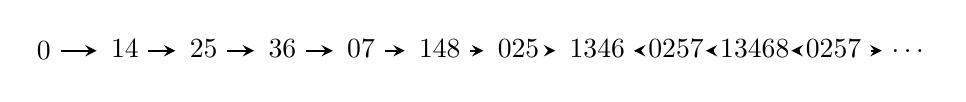
\begin{tikzpicture}[>=stealth, node distance=1cm, every node/.style={sloped}]  % Added slope style for clarity

        % Styles for nodes
        \tikzstyle{state} = []
        
        % Nodes
        \node[state] (0) {0};
        \node[state] (1) [right of=0] {$\begin{matrix} 1 \\ 4 \end{matrix}$};
        \node[state] (2) [right of=1] {$\begin{matrix} 2 \\ 5 \end{matrix}$};
        \node[state] (3) [right of=2] {$\begin{matrix} 3 \\ 6 \end{matrix}$};
        \node[state] (4) [right of=3] {$\begin{matrix} 0 \\ 7 \end{matrix}$};
        \node[state] (5) [right of=4] {$\begin{matrix} 1 \\ 4 \\ 8 \end{matrix}$};
        \node[state] (6) [right of=5] {$\begin{matrix} 0 \\ 2 \\ 5 \end{matrix}$};
        \node[state] (7) [right of=6] {$\begin{matrix} 1 \\ 3 \\ 4 \\ 6 \end{matrix}$};
        \node[state] (8) [right of=7] {$\begin{matrix} 0 \\ 2 \\ 5 \\ 7 \end{matrix}$};
        \node[state] (9) [right of=8] {$\begin{matrix} 1 \\ 3 \\ 4 \\ 6 \\ 8 \end{matrix}$};
        \node[state] (10) [right of=9] {$\begin{matrix} 0 \\ 2 \\ 5 \\ 7 \end{matrix}$};
        \node[state] (11) [right of=10] {\dots};

        % Arrows
        \draw[->, thick] (0) -- (1);
        \draw[->, thick] (1) -- (2);
        \draw[->, thick] (2) -- (3);
        \draw[->, thick] (3) -- (4);
        \draw[->, thick] (4) -- (5);
        \draw[->, thick] (5) -- (6);
        \draw[->, thick] (6) -- (7);
        \draw[->, thick] (7) -- (8);
        \draw[->, thick] (8) -- (9);
        \draw[->, thick] (9) -- (10);
        \draw[->, thick] (10) -- (11);

    
    \end{tikzpicture}
    \caption{sous-classes}
\end{figure}
\end{enumerate}



\begin{exercise}[7.3]
Soit la chaîne de Markov à 10 états $E = \{0, \dots, 9\}$ de matrice de transition :

\[
P =
\begin{pmatrix}
1 & 0 & 0 & 0 & 0 & 0 & 0 & 0 & 0 & 0 \\
0 & \frac{1}{8} & 0 & 0 & \frac{7}{8} & 0 & 0 & 0 & 0 & 0 \\
0 & 0 & 0 & \frac{1}{3} & 0 & 0 & \frac{2}{3} & 0 & 0 & 0 \\
0 & 0 & 0 & 0 & 0 & 0 & 0 & \frac{1}{4} & 0 & \frac{3}{4} \\
\frac{1}{2} & 0 & 0 & 0 & 0 & \frac{1}{2} & 0 & 0 & 0 & 0 \\
0 & \frac{1}{4} & 0 & 0 & \frac{1}{4} & 0 & 0 & \frac{1}{4} & 0 & \frac{1}{4} \\
0 & 0 & \frac{1}{2} & 0 & 0 & 0 & 0 & \frac{1}{2} & 0 & 0 \\
0 & 0 & 0 & 0 & 0 & 0 & 0 & 0 & 1 & 0 \\
\frac{2}{5} & 0 & 0 & 0 & \frac{1}{5} & 0 & 0 & 0 & 0 & \frac{2}{5} \\
0 & 0 & \frac{1}{3} & 0 & 0 & 0 & \frac{1}{3} & 0 & 0 & \frac{1}{3}
\end{pmatrix}.
\]

\begin{enumerate}
    \item \textbf{Tracer son graphe.}
    \item \textbf{Déterminer les classes de la chaîne et leurs périodes.}
\end{enumerate}
\end{exercise}

\subsection*{Solution de l’exercice 7.3}
\begin{enumerate}
    \item Le graphe associé est :

\begin{figure}[h!]
    \centering
    \begin{tikzpicture}[>=stealth, node distance=2cm]

        % Styles for nodes and groups
        \tikzstyle{state} = [circle, draw, fill=red!40, minimum size=0.8cm]
        

        % Nodes
        \node[state] (0) {0};
        \node[state] (5) [right=3cm of 0] {5};
        \node[state] (1) [right=3cm of 5] {1};
        \node[state] (4) [below left=2cm and 1.5cm of 5] {4};
        \node[state] (8) [below left=2cm and 1cm of 1] {8};
        \node[state] (2) [below=5.5cm of 0] {2};
        \node[state] (3) [below=4cm of 5] {3};
        \node[state] (6) [below=2cm of 3] {6};
        \node[state] (7) [below=4cm of 1] {7};
        \node[state] (9) [below=2cm of 7] {9};

       % Groups with custom dimensions
        \node[draw=red, thick, inner sep=0pt, minimum width=2.2cm, minimum height=1.2cm, fit=(0)] {}; 
        
        \node[draw=red, thick, inner sep=0pt, minimum width=6cm, minimum height=2.2cm, fit={(5) (1)}] {};
        
        \node[draw=red, thick, inner sep=0pt, minimum width=6cm, minimum height=2cm, fit={(4) (8)}] {};
        
        \node[draw=red, thick, inner sep=4pt, minimum width=10cm, minimum height=5cm, fit={(2) (3) (6) (7) (9)}] {};


        % Arrows
        \draw[->, thick] (0) edge[loop left] node[left] {1} (0);
        
        \draw[->, thick] (1) edge[loop right] node[right] {$\frac{1}{8}$} (1);
        \draw[->, thick, bend left=25] (5) to node[above] {$\frac{3}{4}$} (1);
        \draw[->, thick, bend left=25] (1) to node[below] {$\frac{7}{8}$} (5);
        \draw[->, thick] (5) edge[loop left] node[left] {$\frac{1}{4}$} (5);
        \draw[->, thick, bend left=25] (4) to node[left] {$\frac{1}{4}$} (5);
        \draw[->, thick, bend left=25] (4) to node[left] {$\frac{1}{2}$} (0);
        \draw[->, thick, bend left=25] (8) to node[right] {$\frac{2}{5}$} (0);
        \draw[->, thick, bend right=25] (8) to node[left] {$\frac{1}{5}$} (5);
    
        \draw[->, thick, bend left=25] (4) to node[above] {$\frac{1}{4}$} (8);
        \draw[->, thick, bend left=25] (8) to node[below] {$\frac{1}{5}$} (4);
        \draw[->, thick] (8) edge[loop right] node[right] {$\frac{1}{5}$} (8);
        

        \draw[->, thick, bend left=25] (2) to node[above] {$\frac{2}{3}$} (6);
        \draw[->, thick, bend left=25] (2) to node[left] {$\frac{1}{3}$} (3);
        \draw[->, thick, bend left=25] (3) to node[above] {$\frac{1}{4}$} (7);
        \draw[->, thick, bend left=25] (6) to node[above] {$\frac{3}{4}$} (9);
        \draw[->, thick, bend left=25] (3) to node[above] {$\frac{3}{4}$} (9);
         \draw[->, thick, bend right=40] (7) to node[below] {\large 1} (2);
        \draw[->, thick, bend left=25] (6) to node[above] {$\frac{1}{4}$} (7);
        \draw[->, thick, bend left=40] (9) to node[below] {\large 1} (2);

    \end{tikzpicture}
\end{figure}



    \item Nous constatons l’existence de 4 classes :
    \begin{itemize}
        \item La classe $\{0\}$, qui est \textbf{fermée} et réduite à un point, formant un état absorbant 0.
        \item La classe $\{1, 5\}$, qui est \textbf{fermée} et \textbf{apériodique}, en raison des boucles en $1$ et $5$.
        \item La classe $\{2, 3, 6, 7, 9\}$, qui est \textbf{fermée} et de \textbf{période 3}. Les 3 sous-classes étant dans l’ordre $\{2\}$, $\{3, 6\}$ et $\{7, 9\}$.
        \item Enfin, la classe $\{4, 8\}$, que nous pouvons quitter vers les classes $\{0\}$ et $\{1, 5\}$, et qui n’est donc pas fermée.
    \end{itemize}

    Nous pouvons voir que nous quittons la classe non fermée $\{4, 8\}$ vers les classes fermées $\{0\}$ et $\{1, 5\}$. Il serait intéressant de savoir avec quelle probabilité nous nous retrouvons dans chacune des deux classes terminales. Or, nous voyons que nous quittons la classe $\{4, 8\}$ de $4$ ou de $8$, et que nous avons toujours deux fois plus de chances de nous retrouver en $0$ que dans la classe $\{1, 5\}$. Par suite, la probabilité de se retrouver en $0$ est $\frac{2}{3}$ et en $\{1, 5\}$ est $\frac{1}{3}$.
\end{enumerate}



\begin{exercise}[7.4]
Déterminer les classes et périodes des exercices suivants du Chapitre 5 :
\begin{itemize}
    \item Exercice 5.4 (marche aléatoire sur $\mathbb{Z}$),
    \item Exercice 5.6 (fort carré),
    \item Exercice 5.7 (transmission d’un bit informatique),
    \item Exercice 5.9 (ruine du joueur),
    \item Exercice 5.10 (plagiste et ses voiliers).
\end{itemize}
\end{exercise}

\subsection*{Solution de l’exercice 7.4}
\begin{itemize}
    \item \textbf{Exercice 5.4 (marche aléatoire sur $\mathbb{Z}$)} : Chaîne irréductible de période 2.
    \item \textbf{Exercice 5.6 (fort carré)} : Chaîne irréductible de période 2, avec comme sous-classes $\{0, 2\}$ et $\{1, 3\}$. De manière générale, la marche aléatoire sur $\mathbb{Z}/n\mathbb{Z}$ est irréductible :
    \begin{itemize}
        \item \textbf{Apériodique} si $n$ est impair,
        \item \textbf{Périodique de période 2} si $n$ est pair.
    \end{itemize}
    \item \textbf{Exercice 5.7 (transmission d’un bit informatique)} : Chaîne irréductible \textbf{apériodique} (car contient des boucles).
    \item \textbf{Exercice 5.9 (ruine du joueur)} : Trois classes :
    \begin{itemize}
        \item $\{0\}$,
        \item $\{N\}$,
        \item $\{1, \dots, N-1\}$.
    \end{itemize}
    Les classes $\{0\}$ et $\{N\}$ consistent en un seul sommet et sont \textbf{fermées}, il s’agit d’états absorbants. La classe $\{1, \dots, N-1\}$ n’est pas fermée, car les classes $\{0\}$ et $\{N\}$ sont accessibles depuis elle. Les deux états absorbants sont de période 1 chacun. La classe non fermée $\{1, \dots, N-1\}$ est de période 2.
    \item \textbf{Exercice 5.10 (plagiste et ses voiliers)} : Chaîne irréductible \textbf{apériodique} (car contient des boucles).
\end{itemize}
